% LaTeX support: latex@mdpi.com
%=================================================================
\documentclass[journal,article,submit,pdftex,moreauthors]{Definitions/mdpi}
%=================================================================
% MDPI internal commands - do not modify
\firstpage{1}
\makeatletter
\setcounter{page}{\@firstpage}
\makeatother
\pubvolume{1}
\issuenum{1}
\articlenumber{0}
\pubyear{2026}
\copyrightyear{2026}
\datereceived{ }
\daterevised{ }
\dateaccepted{ }
\datepublished{ }
\usepackage{graphicx}
\graphicspath{{figures/}}  % Crea carpeta "figures" en Overleaf y sube ahi las imagenes
\usepackage{float}
\usepackage{listings}
\usepackage{xcolor}
\usepackage{tabularx}
\usepackage{booktabs}
\usepackage{amsmath}
%\usepackage{subcaption}    % Para subfiguras (a)(b)

\lstset{
    language=Python,
    basicstyle=\ttfamily\footnotesize,
    keywordstyle=\color{blue},
    stringstyle=\color{red},
    commentstyle=\color{green!50!black},
    showstringspaces=false,
    frame=single,
    breaklines=true
}
%=================================================================
\Title{Real-Time Intelligent Energy Management System for Microgrid Operation}
\Author{David D\'iaz $^{1,\dagger,*}$, Dar\'io Solarte $^{1,\dagger}$, Javier Revelo-Fuelag\'an $^{1,\dagger}$}
\AuthorNames{David D\'iaz, Jefersson Solarte, Javier Revelo-Fuelagán}
\address{%
$^{1}$ \quad Department of Electronics, Faculty of Engineering, Universidad de Nari\~no, Pasto, Colombia; dsdiazhack666@udenar.edu.co; dariosolarte12@udenar.edu.co; javierrevelof@udenar.edu.co}
\corres{Correspondence: david.diaz@udenar.edu.co}

\abstract{The increasing penetration of intermittent renewable sources, along with the operational complexity of storage systems and conventional generation, demands advanced energy management tools. This work presents the Intelligent Energy Management System (SIGE), a comprehensive platform for the operation of hybrid microgrids that integrates low-latency IoT monitoring, time-series forecasting, stochastic optimization with model predictive control (MPC), multidimensional statistical anomaly detection, and a multi-agent system based on large language models (LLMs). The platform operates autonomously in a continuous cycle where it acquires data via the MQTT protocol, obtains solar irradiance and energy demand forecasts from stored historical series, and performs the economic dispatch management of a microgrid in Pyomo with Gurobi. The results demonstrate the viability of a hybrid architecture that integrates mathematical optimization with artificial intelligence, offering a tool for microgrid operation that integrates distributed generation from non-conventional energy sources.}

\keyword{Microgrids; Intelligent Management; Model Predictive Control (MPC); Stochastic Optimization; LLM Agents; IoT.}
%%%%%%%%%%%%%%%%%%%%%%%%%%%%%%%%%%%%%%%%%%
\begin{document}
%%%%%%%%%%%%%%%%%%%%%%%%%%%%%%%%%%%%%%%%%%
\section{Introduction}

Microgrids, which are generation, storage, and consumption systems that can operate isolated or interconnected with the main grid, represent a fundamental paradigm in the energy transition. However, their efficient operation faces considerable challenges: solar photovoltaic generation is inherently intermittent and depends on variations in meteorological conditions; diesel generators, although dispatchable, present non-linear operational costs and environmental externalities; batteries introduce temporal dynamics between consecutive periods; and the external power grid involves exchange restrictions and variable tariffs \cite{ref-alternar}.

Decision-making in this context requires continuously solving a multi-period optimization problem under uncertainty, fed by real data from energy meters and projections of future conditions. Traditional solutions based on heuristic rules or simple deterministic optimization do not adequately capture the stochastic nature of renewable sources nor do they leverage the temporal granularity offered by modern data acquisition systems \cite{ref-carrasco}.

Therefore, the SIGE platform is developed for the optimal operation of microgrids that integrates the following functionalities: (1) real-time acquisition and monitoring of electrical variables through smart energy meters installed in the microgrid and connected using IoT technology, utilizing the MQTT protocol for data transmission and MongoDB for scalable persistence; (2) multi-horizon time-series forecasting of solar irradiance and load demand, allowing the progressive integration of machine learning models, including a Temporal Fusion Transformer (TFT) model trained offline; (3) stochastic optimization with model predictive control (MPC), solving an economic energy dispatch problem that considers multiple weather scenarios weighted by probability, with a 24-hour horizon and hourly resolution; (4) real-time anomaly detection using three complementary statistical strategies (thresholds, rate of change, contextual Z-score), which feed a multi-agent system based on LLMs to generate diagnostics and operational recommendations in natural language; and (5) an interactive operator interface that includes a single-line diagram editor, graphical visualization of dispatch plans, real-time monitoring of energy meters, and dynamically AI-generated dashboards. The central objective of the platform is to become a real-time analysis system that, using real data from the microgrid's components, predicts future conditions and autonomously optimizes its operation, ensuring the reduction of operational costs and maximizing supply reliability.

Intelligent microgrid management has been addressed from various fronts, highlighting energy time-series forecasting. While models like ARIMA and LSTM networks show more accurate results in short horizons, they present difficulties in processing long-term dependencies and complex exogenous variables. As an alternative, the Temporal Fusion Transformer (TFT) \cite{ref-lim} introduces attention mechanisms and adaptive gating, facilitating multi-horizon predictions with uncertainty quantiles; a critical capability for forecasting renewable generation and electrical demand \cite{ref-rao,ref-tasmant}.

Regarding optimal microgrid operation, stochastic programming has been widely used to model uncertainty in renewable generation and demand \cite{ref-birge,Parisio2014,Su2014,Zia2018,Hua2019}. Model predictive control (MPC) \cite{ref-rawlings} complements this approach by implementing a receding horizon strategy that periodically recalculates the optimal solution, adapting to new real-time information. Tools like Pyomo \cite{ref-bynum} facilitate the algebraic formulation of these problems, while solvers like Gurobi \cite{ref-gurobi} and HiGHS \cite{ref-huangfu} allow for their efficient resolution.

On the front of artificial intelligence applied to electrical infrastructure supervision, large language models (LLMs) have begun to be integrated as cognitive assistants for operators. Frameworks like LangChain \cite{ref-chase} and LangGraph allow the orchestration of multi-agent workflows that process energy meter data, detect anomalous patterns, and generate diagnostics in natural language. However, the integration of these three dimensions—forecasting, stochastic optimization, and AI agents—in a platform that operates in a closed loop on real data from the microgrid constitutes a gap that this work seeks to address \cite{ref-lami}.

Beyond economic optimality, recent work emphasizes resilient operation under cyber-physical disturbances. Han et al. \cite{Han2026} propose a resilient optimal dispatch strategy for ship-integrated energy systems based on an enhanced traffic jam optimizer, addressing degraded operating conditions and false-data injections. In SIGE, resilience is addressed at the data layer: the multidimensional statistical anomaly detection described in Section~2.2 and the LLM-based supervisory layer identify compromised or erroneous measurements before they propagate into the optimization loop, complementing the economic dispatch with a security-aware operating envelope.

In this context, this research work presents the following contributions: first, the implementation of a TFT model trained with real data from IoT meters and meteorological variables; second, the integration of multi-horizon predictions into a stochastic MPC control loop, which allows for a reduction in operational costs compared to deterministic strategies; and third, the development of a multi-agent system based on LLMs capable of processing statistical anomaly analyses to provide real-time operational assistance without human intervention. The relationship between the identified research gaps and the contributions of this work is summarized in Table~\ref{tab:related}.

\begin{table}[H]
\centering
\caption{Synthesis of related work, research gaps, and SIGE contributions.}
\label{tab:related}
\begin{tabularx}{\textwidth}{p{2.2cm}p{1.7cm}p{2.5cm}p{2.5cm}X}
\toprule
\textbf{Reference} & \textbf{Area} & \textbf{Method} & \textbf{Limitation (gap)} & \textbf{How SIGE addresses it} \\
\midrule
\cite{ref-lim,ref-rao,ref-tasmant} & Forecasting & TFT / ARIMA / LSTM multi-horizon & Not embedded in the control loop & Modular TFT predictor feeding MPC scenarios \\
\cite{ref-birge,ref-rawlings,Parisio2014,Su2014,Zia2018,Hua2019} & Stochastic opt.\ \& MPC & Scenario-based uncertainty + receding horizon & Evaluated offline / in isolation & Closed-loop MPC on real IoT data, 15-min recompute \\
\cite{ref-lami,ref-chase} & LLM infrastructure & Multi-agent orchestration & No safety envelope for control & Advisory-only LLM: allowlist + numeric verification + audit \\
\cite{Han2026} & Resilience & Resilient dispatch under attacks & Focused on ship-integrated systems & Data-layer resilience: anomaly detection + LLM supervision \\
\cite{ref-carrasco} & Heuristics & Rule-based dispatch & No stochastic capture & Stochastic MPC with probabilistic scenarios \\
\cite{ref-alternar} & Microgrid paradigm & Context & Motivates scope & SIGE hybrid closed-loop scope \\
\midrule
This work & -- & -- & -- & Hybrid closed-loop platform (IoT + forecasting + stochastic MPC + LLM supervision) on real microgrid data \\
\bottomrule
\end{tabularx}
\end{table}

This paper is structured as follows: Section 1 introduces the microgrid paradigm and outlines the development of the SIGE platform. Section 2 details the methodology, describing the multilayer technological architecture that integrates IoT instrumentation, the Temporal Fusion Transformer (TFT) prediction model, the stochastic optimization loop (MPC), and the multi-agent system based on LLMs for anomaly detection and operational assistance. Subsequently, Section 3 presents the experimental results obtained during system validation, including performance metrics and the analysis of the microgrid's behavior. Finally, Section 4 discusses the scope and limitations of the study, culminating with the conclusions that validate the viability of this hybrid approach for autonomous decision-making in distributed energy infrastructure.

%%%%%%%%%%%%%%%%%%%%%%%%%%%%%%%%%%%%%%%%%%
\section{Materials and Methods}

SIGE is organized into three technological layers that communicate via REST APIs, WebSockets, Redis, and MQTT, as shown in Figure~\ref{fig:arquitectura}:

\begin{figure}[H]
    \centering
    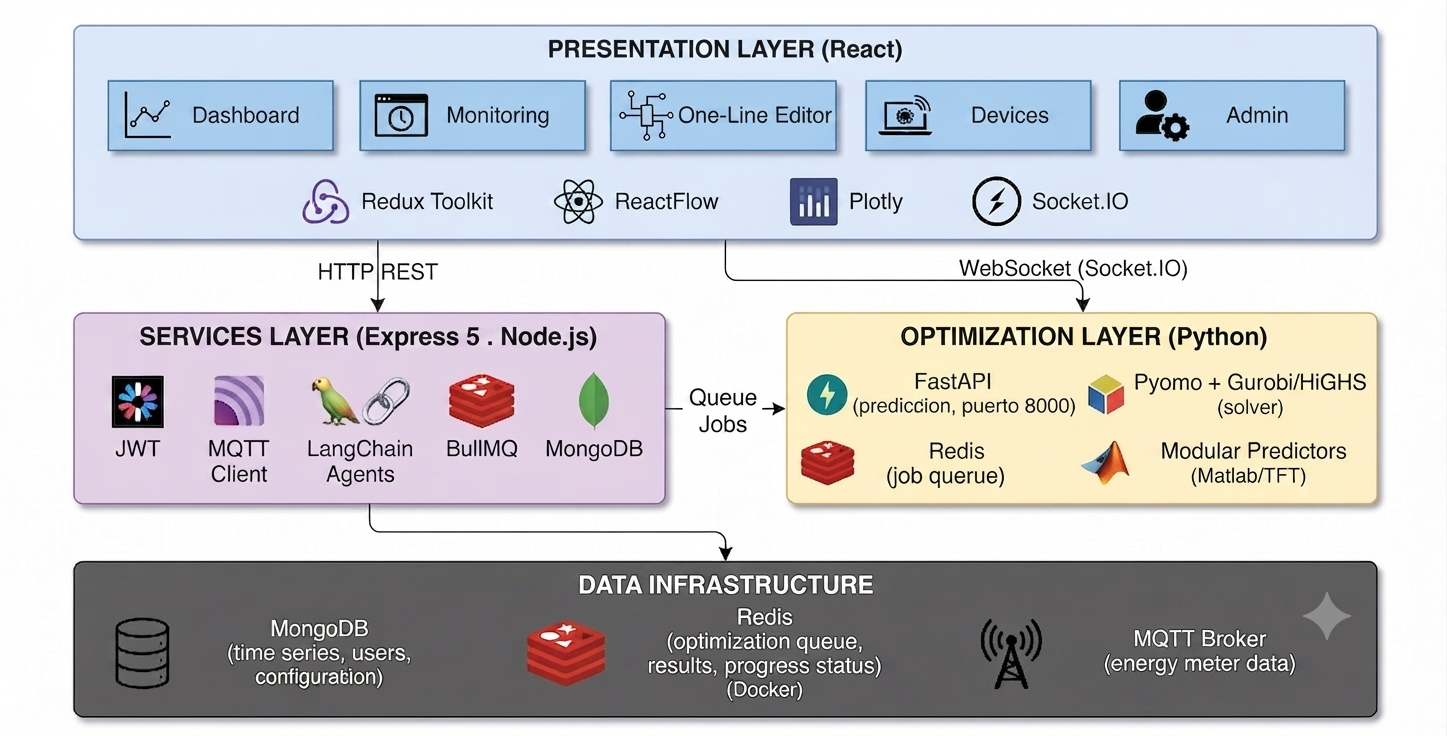
\includegraphics[width=\textwidth]{ENGimages/arquitectura.png} 
    \caption{Multilayer technological architecture of the SIGE system.}
    \label{fig:arquitectura}
\end{figure}

The first layer corresponds to the implementation of functional modules accessible via tabbed navigation: Optimization Dashboard, Real-time Monitoring, Single-line Diagram Editor, IoT Device Management, AI-generated Dashboard (server-driven UI), and Operator Administration. The application state is managed using Redux Toolkit, with specialized reducers. Real-time communication with the backend is carried out via Socket.IO, while CRUD operations use a REST API with JWT authentication.

The service layer, running on Node.js with Express 5, acts as the central orchestrator and performs the following functions: manages authentication, maintains the connection with the MQTT broker for data ingestion, coordinates MPC cycles, executes the AI agent pipeline, and serves as a bridge with Python services.

The optimization layer, implemented in Python, contains two independent services: a FastAPI API that exposes forecasts generated by modular predictors and a Pyomo-based resolution engine that builds and solves the stochastic economic dispatch model using Gurobi as the main solver, with HiGHS as an open-source alternative. The data flow in the platform follows a continuous pipeline divided into two main circuits, shown in Figure~\ref{fig:flujo de datos}:

\begin{figure}[H]
    \centering
    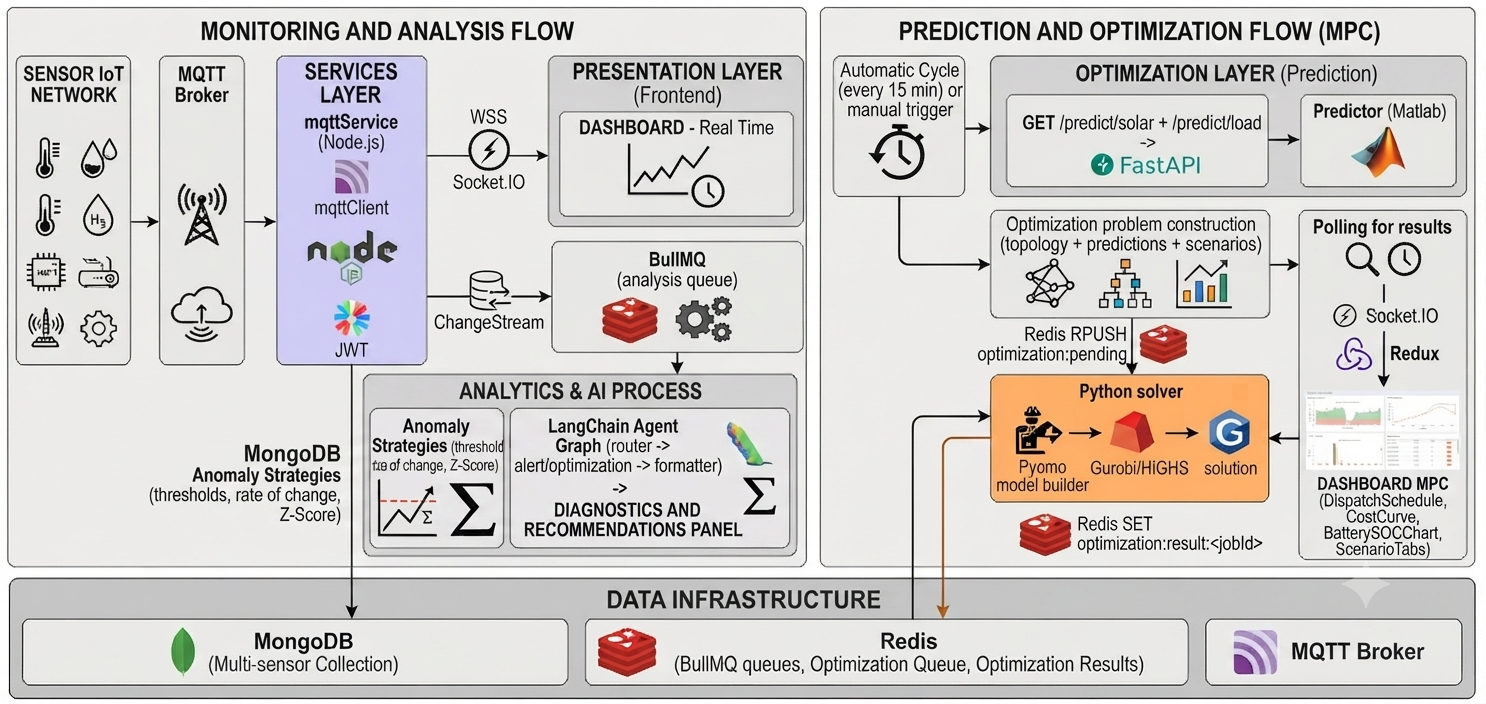
\includegraphics[width=\textwidth]{ENGimages/flujo_de_datos.png} 
    \caption{Data flow}
    \label{fig:flujo de datos}
\end{figure}


The platform connects to an external MQTT broker to which the energy meters installed in the microgrid are linked. These devices publish their measurements to specific topics and the system maintains an active subscription to authorized topics, allowing it to receive energy meter readings in real time \cite{ref-medicion}.

Validated data is persisted in MongoDB using a dynamic storage model, where each device has its own partitioned collection. This strategy facilitates time-series queries and allows the establishment of differentiated retention policies depending on the nature of the sensor. Simultaneously, each reading is transmitted to the frontend using rooms; this allows updating the monitoring graphs with sub-second latencies. Figure~\ref{fig:monitoreo} shows the real-time monitoring interface with energy meter readings.

% ------------------------------------------------------------------
% FIGURA: M\'odulo de monitoreo IoT en tiempo real
% Sube a Overleaf: figures/ui_monitoreo_iot.png
% ------------------------------------------------------------------
\begin{figure}[H]
    \centering
    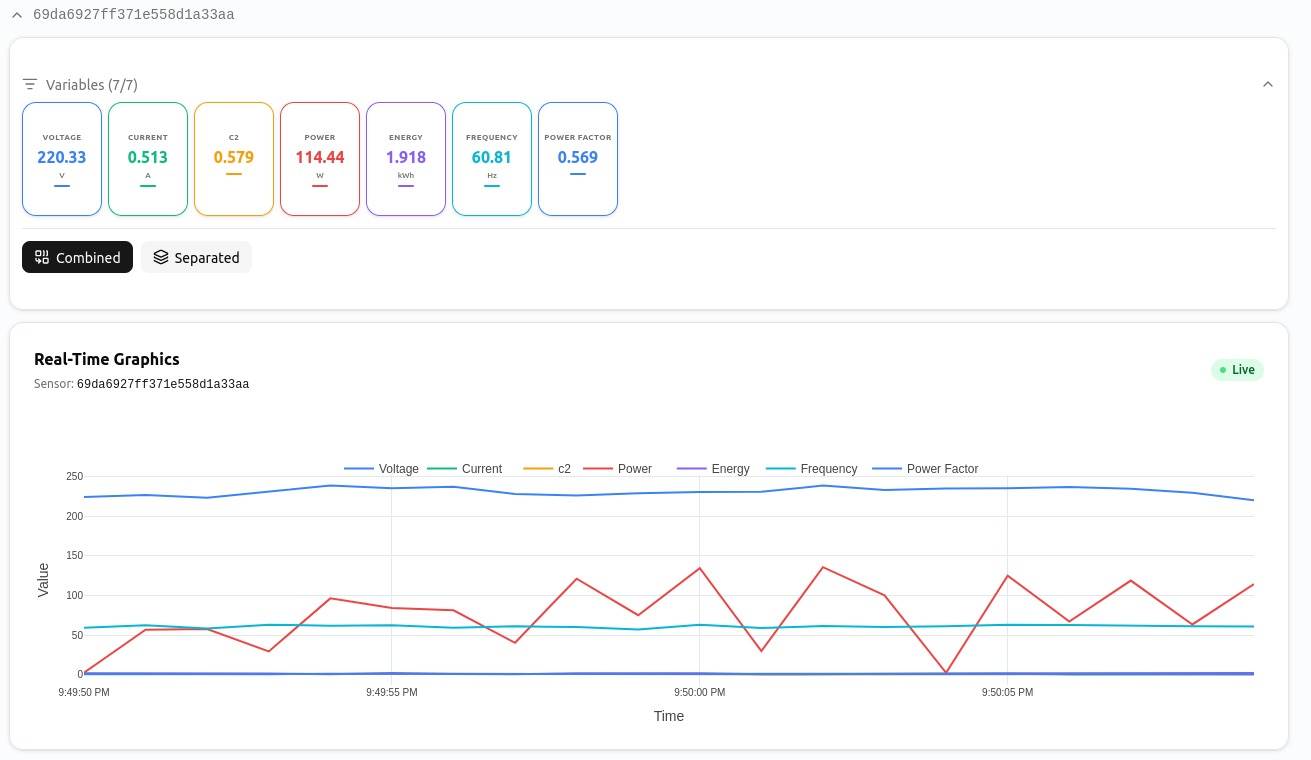
\includegraphics[width=\textwidth]{ENGimages/ui_monitoreo_iot.jpeg}
    \caption{Real-time monitoring module with energy measurement logging.}
    \label{fig:monitoreo}
\end{figure}
% ------------------------------------------------------------------


The \textit{ChangeStream} functionality of MongoDB allows the platform to detect every new insertion without the need for periodic polling. The \texttt{changeStreamService} maintains open cursors on all active collections, queuing data asynchronously in the Node.js BullMQ library.
\\


Regarding the forecasting system, the platform integrates a modular interface that decouples the forecasting engine from the rest of the system, allowing the modular implementation of various algorithms without altering backend orchestration.

For production execution, the system implements an API developed in FastAPI that decouples the prediction engine from the rest of the platform. This architecture allows incorporating and substituting different forecasting models seamlessly, without requiring modifications to the orchestration flow or the other system components.

Currently, the platform has two implementations compatible with this interface. The first corresponds to MatlabPredictor, used during the system's current operation via preprocessed historical time series. The second corresponds to TFTPredictor, developed as an alternative implementation aimed at integrating a model based on the Temporal Fusion Transformer.

The TFT model was trained using an independent pipeline that uses data from the microgrid's energy meters and external meteorological variables. This training process comprises the acquisition of time series from MongoDB and the Open-Meteo API over a twenty-day period, followed by preprocessing that included hourly resampling and the calculation of derived variables. Finally, a multi-horizon configuration was executed to forecast twenty-four future steps, after which the model was serialized for future integration into the production environment.
\\
The TFT architecture allows the handling of multiple exogenous variables, the generation of probabilistic forecasts via uncertainty quantiles, and the use of attention mechanisms to weight the relevance of historical variables. The integration of these uncertainty quantiles into the model predictive control (MPC) loop replaces the current deterministic approach with a stochastic one that allows optimizing decision-making under conditions of climate variability.

\subsection{Stochastic optimization and model predictive control}

The mathematical core of SIGE is a stochastic economic dispatch problem formulated as a quadratic program with continuous variables. The formulation covers a 24-period (hour) time horizon and explicitly handles uncertainty.
\\\\
The optimization model bases its operational decisions on a set of variables that are evaluated hour by hour under different stochastic scenarios. To ensure supply, the system determines the exact amount of power (in kW) that each available diesel unit must generate. Similarly, the model calculates the power exchange with the main grid, dynamically identifying when it is necessary to import energy from the outside to cover internal demand.
\\\\
Regarding storage management, the system controls the bidirectional flows of the batteries. The model defines the net charge and discharge power required in each period to optimize the use of available resources. As a result of these energy transfers, the system monitors the state of charge of each battery at the end of each hour, which is measured in kWh, thus ensuring precise tracking of the accumulated energy and respecting the physical limits of the equipment.
\\
Solar generation is modeled as a pre-calculated stochastic parameter based on irradiance predictions and scenario factors, injected directly into the power balance constraint. 

Energy management in the microgrid is posed as an optimization problem that minimizes the total operating cost, as shown in Equation (1), weighted by the probabilities of each scenario, including quadratic cost functions for the diesel generator, grid tariffs, and linear penalties for battery degradation:
\begin{equation}
\min \sum_{s} \text{prob}[s] \cdot \sum_{t} \left[ \sum_{d} (c_d + b_d P_d + a_d P_d^2) C_{\text{comb}} + (C_{\text{fijo}} + C_{\text{var}} P_{\text{grid}}) + \sum_{b} \text{deg} (P_{\text{ch}} + P_{\text{dis}}) \right]
\end{equation}

The solution space is bounded by the power balance, defined as $\Sigma P_{\text{diesel}} + P_{\text{grid}} + P_{\text{solar}} + \Sigma P_{\text{discharge}} - \Sigma P_{\text{charge}} \ge P_{\text{load}}$, as well as by the operational limits of the diesel generators, expressed by $P_{\text{min}}[d] \le P_{\text{diesel}}[d,t,s] \le P_{\text{max}}[d]$. Additionally, the system is subject to power grid constraints, $P_{\text{grid\_min}} \le P_{\text{grid}}[t,s] \le P_{\text{grid\_max}}$, and battery state of charge limits, defined by $SOC_{\text{min}}[b] \le SOC[b,t,s] \le SOC_{\text{max}}[b]$.
\\

Battery dynamics are presented by equations (2) and (3), which describe the temporal evolution of the state of charge (SOC) of each battery over the optimization horizon. These relationships consider charge and discharge efficiencies, the initial state of charge, and the intertemporal coupling between consecutive periods.


    \begin{align}
        SOC[b,0,s] &= SOC_{\text{ini}}[b] + \eta_{\text{ch}}[b] \cdot P_{\text{ch}}[b,0,s] - \frac{P_{\text{dis}}[b,0,s]}{\eta_{\text{dis}}[b]} \\
        SOC[b,t,s] &= SOC[b,t-1,s] + \eta_{\text{ch}}[b] \cdot P_{\text{ch}}[b,t,s] - \frac{P_{\text{dis}}[b,t,s]}{\eta_{\text{dis}}[b]}, \quad t > 0
    \end{align}
Although the objective function already penalizes simultaneous charge and discharge through the degradation term $\text{deg} > 0$, an explicit complementarity constraint is imposed to guarantee physical feasibility. Binary indicators $y_{\text{ch}}[b,t,s], y_{\text{dis}}[b,t,s] \in \{0,1\}$ enforce that at most one operation mode is active per battery, period, and scenario:
    \begin{align}
        y_{\text{ch}}[b,t,s] + y_{\text{dis}}[b,t,s] &\le 1 \\
        P_{\text{ch}}[b,t,s] &\le P_{\text{ch,max}}[b] \cdot y_{\text{ch}}[b,t,s] \\
        P_{\text{dis}}[b,t,s] &\le P_{\text{dis,max}}[b] \cdot y_{\text{dis}}[b,t,s]
    \end{align}



\subsubsection{Resolution and predictive control loop (MPC)}
The problem is solved using Gurobi as the main solver, with HiGHS as an open-source alternative for user selection. The closed MPC loop automatically recalculates the full 24-hour horizon every 15 minutes, implementing only the action of the first time period according to the receding horizon strategy. Communication between the Node.js backend and the Python solver is done via Redis. The backend queues optimization jobs in a shared list within Redis, and the solver consumes them for processing; once the model is solved, the results and progress state are stored in the same Redis server, from where the backend retrieves them through periodic polling.

\subsection{Anomaly detection and AI multi-agent system}
The statistical detection strategies employed establish that each meter reading is subjected to three complementary analyses executed in parallel:
\begin{enumerate}
    \item \textbf{Threshold strategy:} Verifies that each electrical variable is within predefined physical ranges, with configurable limits by device type (solar panels, inverters, batteries, meters, microgrid).
    \item \textbf{Rate of change:} Calculates the relative variation between consecutive readings $|(x_t - x_{t-1}) / x_{t-1}|$. To avoid division by zero when the previous reading is null (e.g., photovoltaic power at night), the strategy switches to an absolute-difference test $|x_t - x_{t-1}|$ compared against an absolute threshold specific to each variable, instead of forcing a spurious 100\% jump. Thresholds are defined per variable type with physical justification: voltage $\pm 10\%$ (grid regulation), active/reactive power $\pm 50\%$ (normal PV and demand ramps), current $\pm 50\%$, and state of charge $\pm 20\%$ (bounded by the battery management system); unclassified variables fall back to a 50\% relative threshold. This design prevents false positives during null-base transitions while preserving sensitivity to genuine abrupt changes.
    \item \textbf{Contextual Z-score:} Evaluates each reading against the mean and standard deviation of a rolling historical window (30 readings by default), flagging values with $|Z| > 3.0$.
\end{enumerate}

A strategy log aggregates the results of the three techniques and assigns an alert level: \texttt{Critical} when two or more strategies detect an anomaly, \texttt{Warning} when only one detects it, and \texttt{Normal} in the absence of signals.

\subsubsection{Multi-agent system based on LLMs}
SIGE integrates a cognitive system implemented with \textbf{LangChain} and \textbf{LangGraph} that processes the statistical analysis results and acts as an operator copilot. The state graph contains four specialized nodes:
\begin{itemize}
    \item \textbf{Router:} Evaluates the presence of anomalies in the previous analysis and routes the flow to the alert or optimization node accordingly.
    \item \textbf{Alert:} Under anomalous conditions, invokes the LLM (Llama 3.3 70B via Groq, or GPT-4o-mini via OpenAI as an alternative) to generate a diagnostic summary and actionable recommendations.
    \item \textbf{Optimization:} In a normal operating state, the LLM suggests guidelines for preventive maintenance and operational efficiency.
    \item \textbf{Formatter:} Structures the final response with visualization data for the frontend.
\end{itemize}

The LLM responses are validated against \texttt{Zod} schemas to ensure their structural integrity before being transmitted to the frontend via Socket.IO. Beyond structural validation, the system enforces a multi-layer safety design: (i) the LLM is strictly advisory and is never granted the ability to execute control actions---its output is a recommendation that the physical control loop executes exclusively through the MPC and human operator confirmation, so the LLM remains outside the control data path; (ii) an allowlist restricts the recommended action types to those predefined by the system; (iii) numerical verification checks that any suggested setpoint lies within physically admissible ranges derived from the input data; and (iv) every recommendation is logged with its justification to support traceability and audit. In the operator interface, recommendations are presented as suggestions that require operator confirmation before any effect.

\subsection{Operator interface}
The platform includes a single-line diagram editor implemented with \textbf{ReactFlow} that allows operators to build and modify the microgrid's topology using configurable nodes (solar panel, diesel generator, power grid, inverter, battery, and load). The topology defined in the editor is automatically translated into solver constraints when triggering an optimization. Each diagram node maps to its corresponding entry in the \texttt{sources}, \texttt{storage}, \texttt{loads}, or \texttt{grid} arrays consumed by the Pyomo model. Figure~\ref{fig:editor} shows the single-line diagram editor of a grid topology.

% ------------------------------------------------------------------
% FIGURA E: Editor de diagrama unifilar (ReactFlow)
% Sube a Overleaf: figures/ui_editor_unifilar.png
% ------------------------------------------------------------------
\begin{figure}[H]
    \centering
    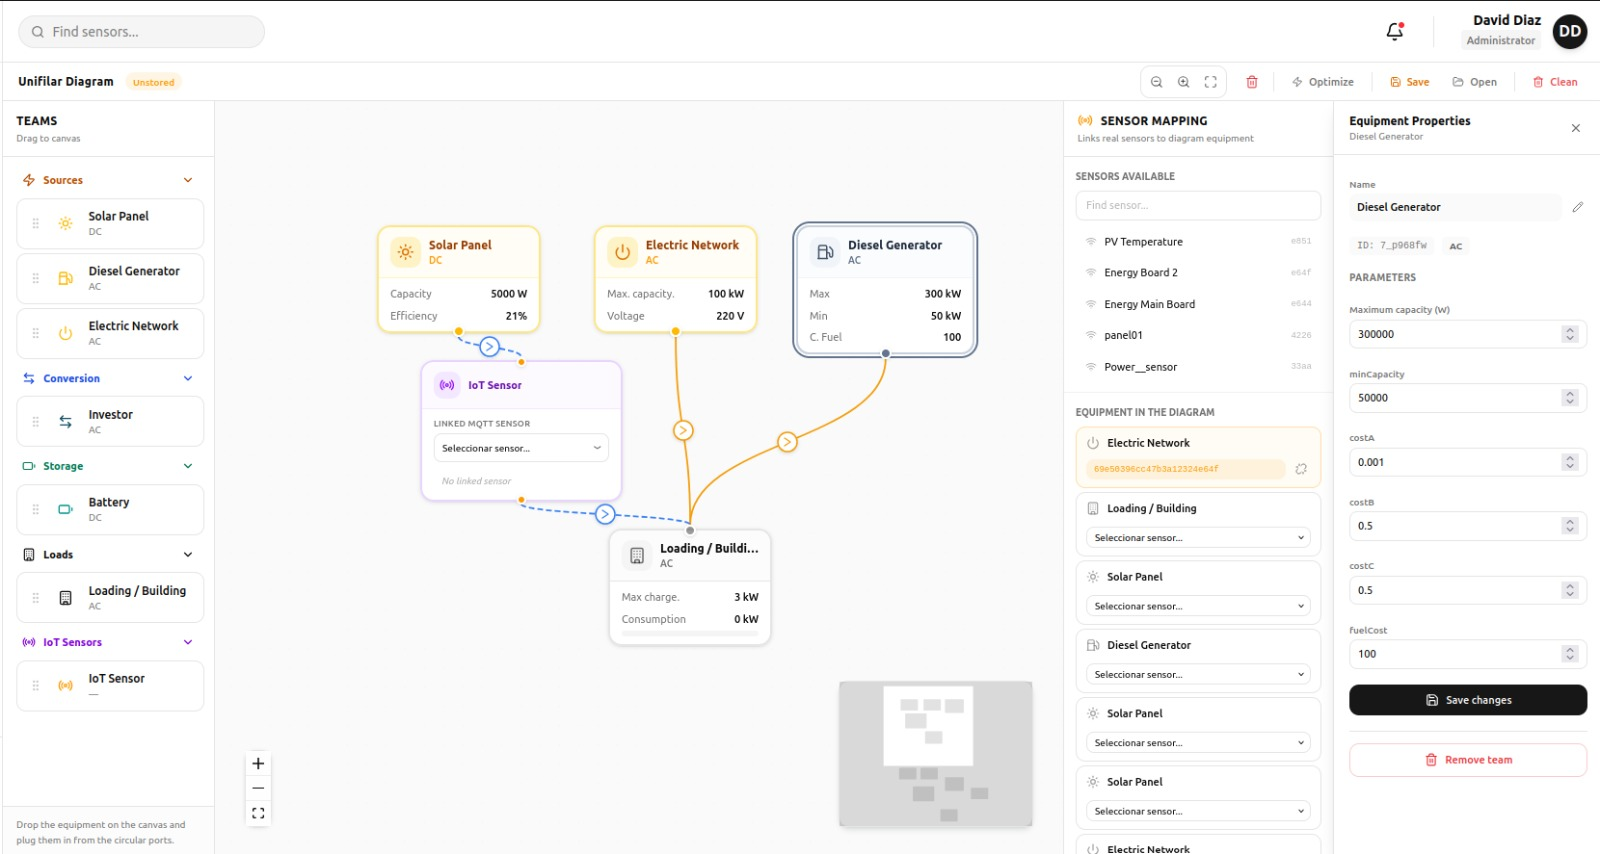
\includegraphics[width=\textwidth]{ENGimages/ui_editor_unifilar.png}
    \caption{Single-line diagram editor that is automatically converted into solver constraints.}
    \label{fig:editor}
\end{figure}
% ------------------------------------------------------------------


\subsubsection{AI-generated dashboard and multi-agent analysis}
SIGE offers complementary features powered by artificial intelligence. Specifically, the Server-Driven Dashboard module employs an LLM (Groq/OpenAI) to dynamically generate a JSON dashboard specification. This specification defines widgets (metric cards, energy meter tables, line and bar charts) that are rendered with real data from the user's authorized energy meters. In the absence of an LLM API key, the system produces a default dashboard based on the latest available readings. Figure~\ref{fig:dashboard_ia} shows the AI agent console with real-time analysis and recommendations generated by the LangGraph graph.

% ------------------------------------------------------------------
% FIGURA I: Dashboard Server-Driven UI generado por IA
% Sube a Overleaf: figures/ui_dashboard_ia.png
% ------------------------------------------------------------------
\begin{figure}[H]
    \centering
    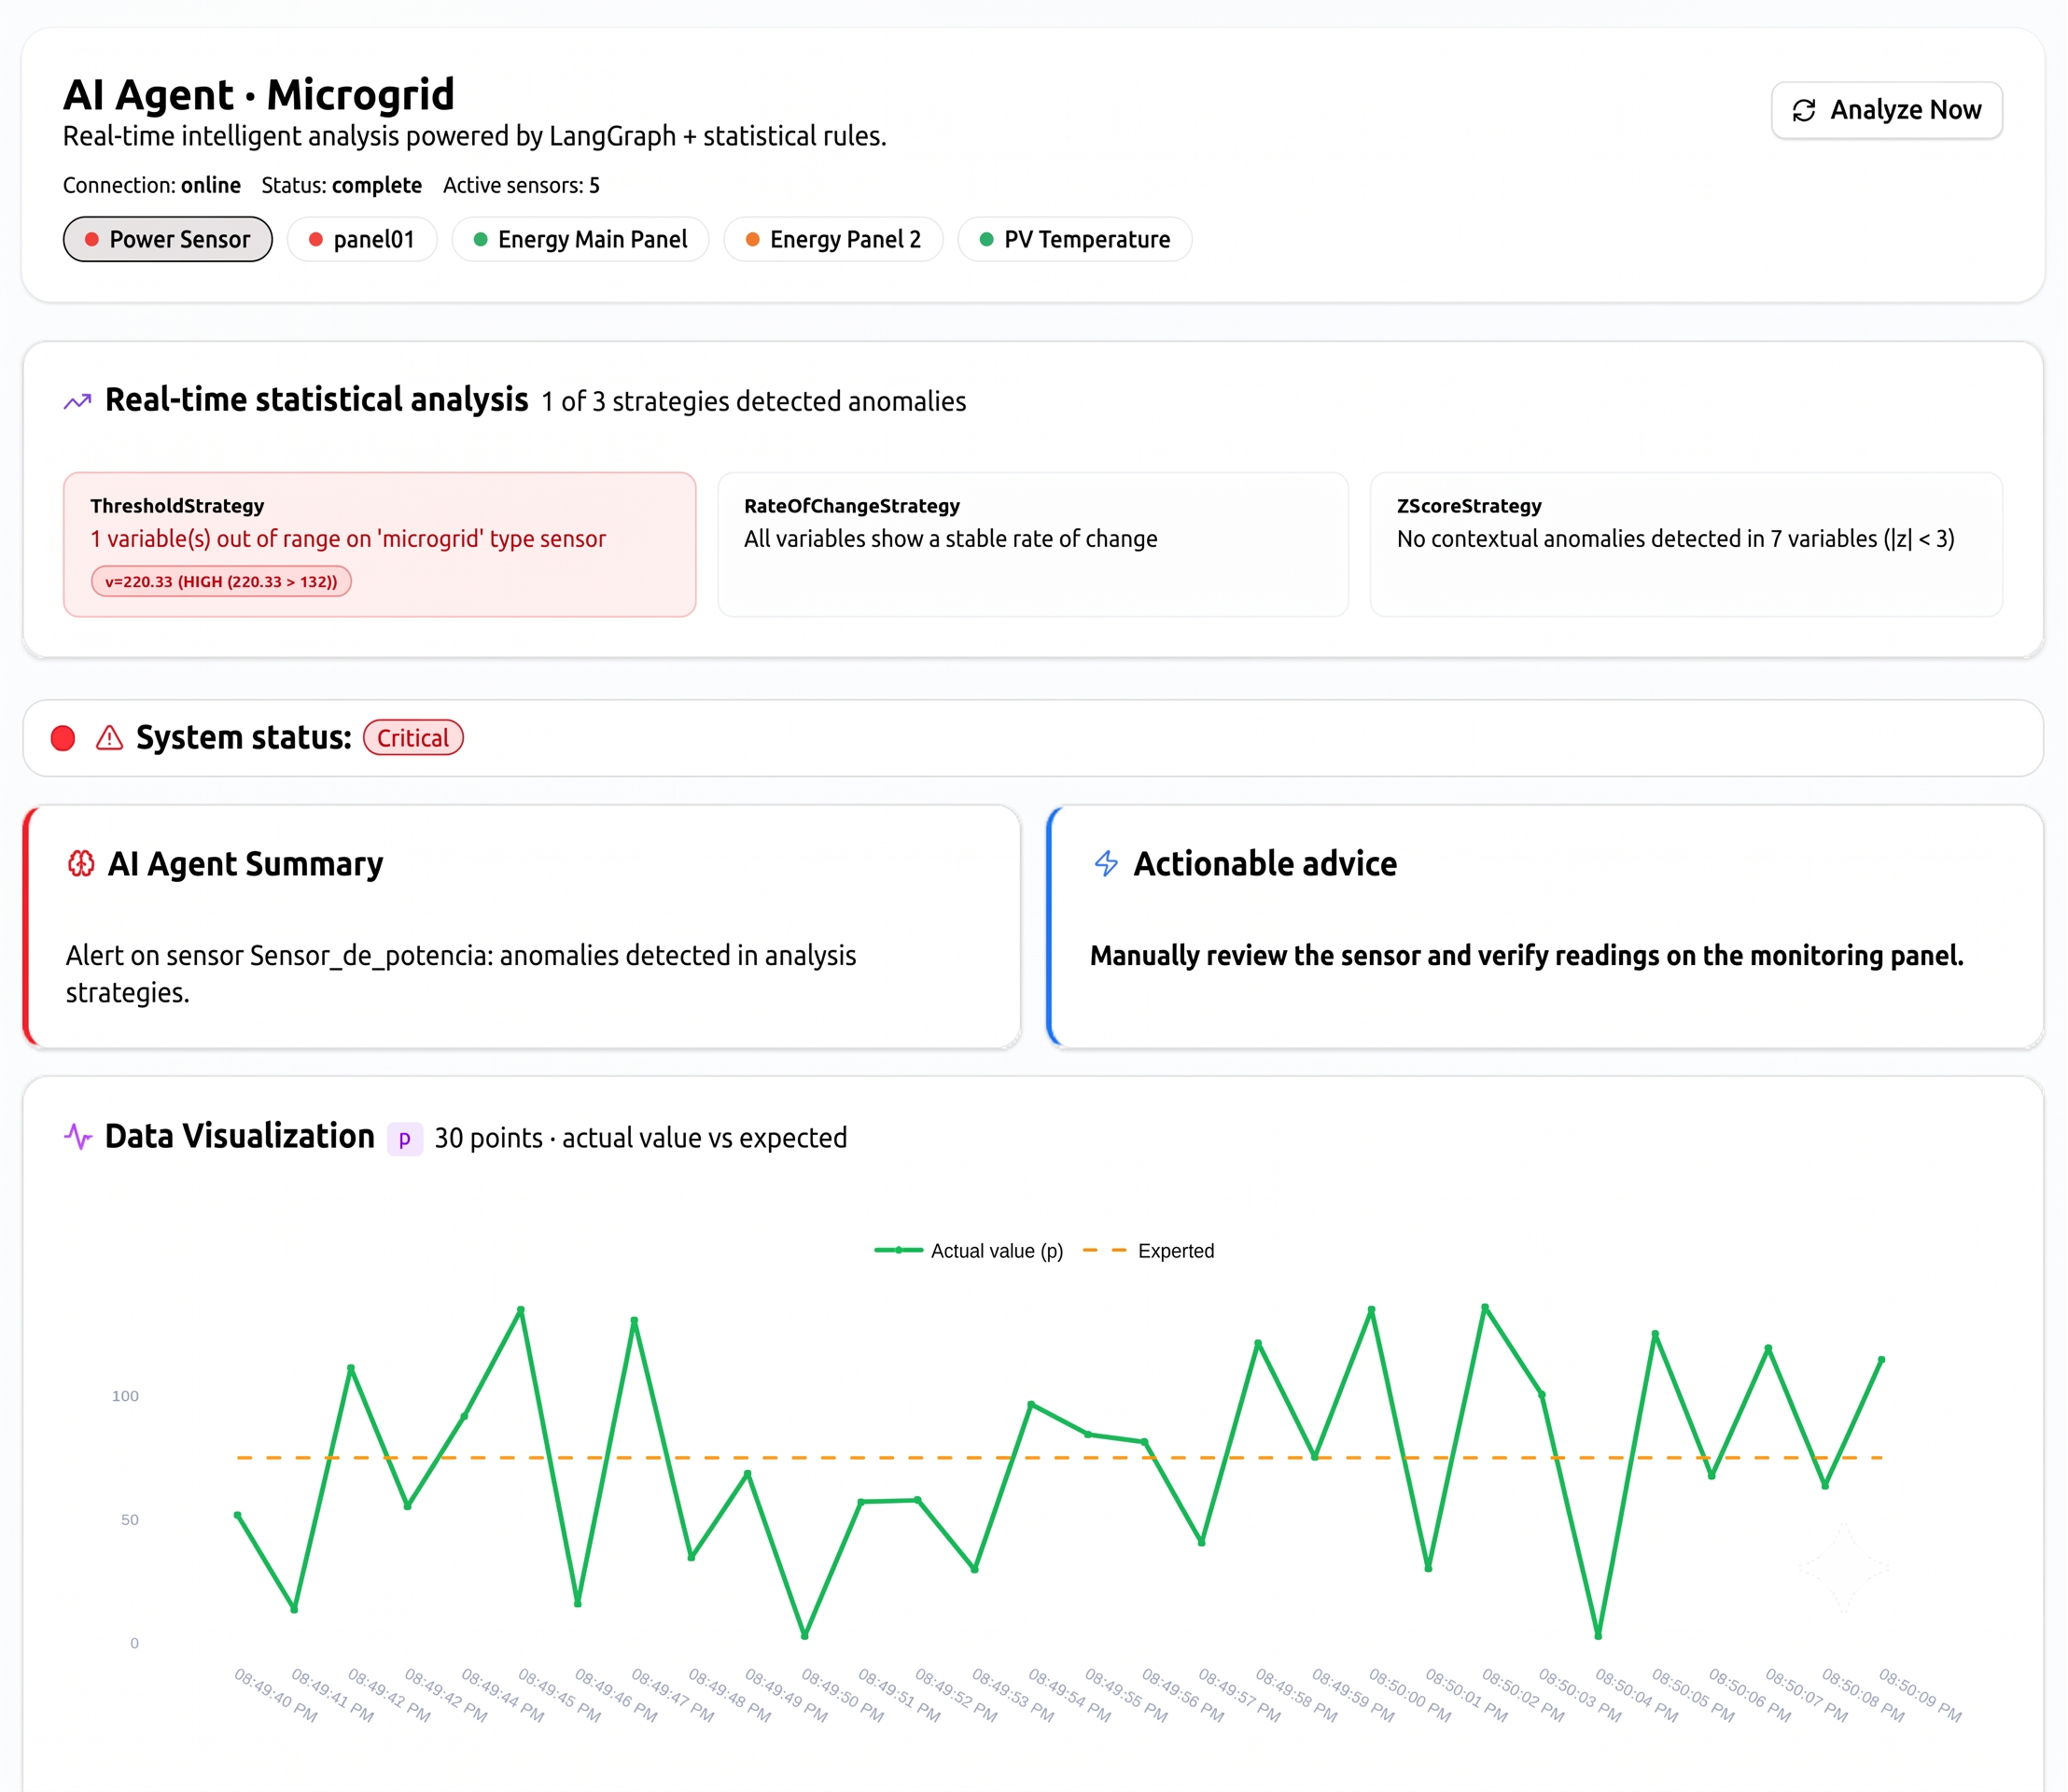
\includegraphics[width=0.90\textwidth]{ENGimages/ui_dashboard_ia.png}
    \caption{AI agent Server-Driven UI console.}
    \label{fig:dashboard_ia}
\end{figure}
% ------------------------------------------------------------------
%%%%%%%%%%%%%%%%%%%%%%%%%%%%%%%%%%%%%%%%%%

\section{Results}

The experimental validation of SIGE was conducted through a case study of a hybrid microgrid integrating IoT energy meters. The obtained results are presented following the functional flow of the SIGE platform. Initially, the configuration used during the validation is described, followed by an analysis of the optimization cycle results, then the performance of the prediction model, and finally, the functional integration of the different modules that make up the system.


Figure~\ref{fig:topologia} presents the topology used during the experimental validation of the system. The considered microgrid consists of photovoltaic panels, a diesel generator, three electrical loads, and the connection to the main grid. This microgrid was configured on the platform using the single-line diagram editor and subsequently automatically translated to the optimization model implemented in Pyomo.

\begin{figure}[H]
    \centering
    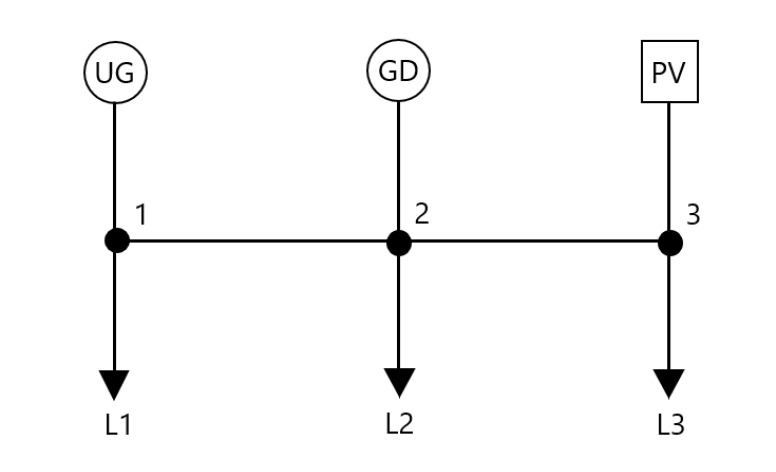
\includegraphics[width=0.85\textwidth]{images/Driagrama_unifilar_microrred.jpeg}
    \caption{Microgrid topology used for system validation.}
    \label{fig:topologia}
\end{figure}

The topology constitutes the scenario used to evaluate the predictive control cycle and verify the integration between the graphical editor, the mathematical model, and the optimization engine.
\\
The obtained result shows the power distribution among the available sources during the optimization horizon and the projected evolution of the batteries' state of charge. Operational indicators used to monitor each execution cycle are also generated from this solution.
\\
Figure~\ref{fig:dashboard_opt} presents the result of an optimization cycle executed over a 24-hour prediction horizon. The dashboard shows the optimal power dispatch obtained for the different generation sources and the expected cost associated with the scenarios considered by the model.

\begin{figure}[H]
    \centering
    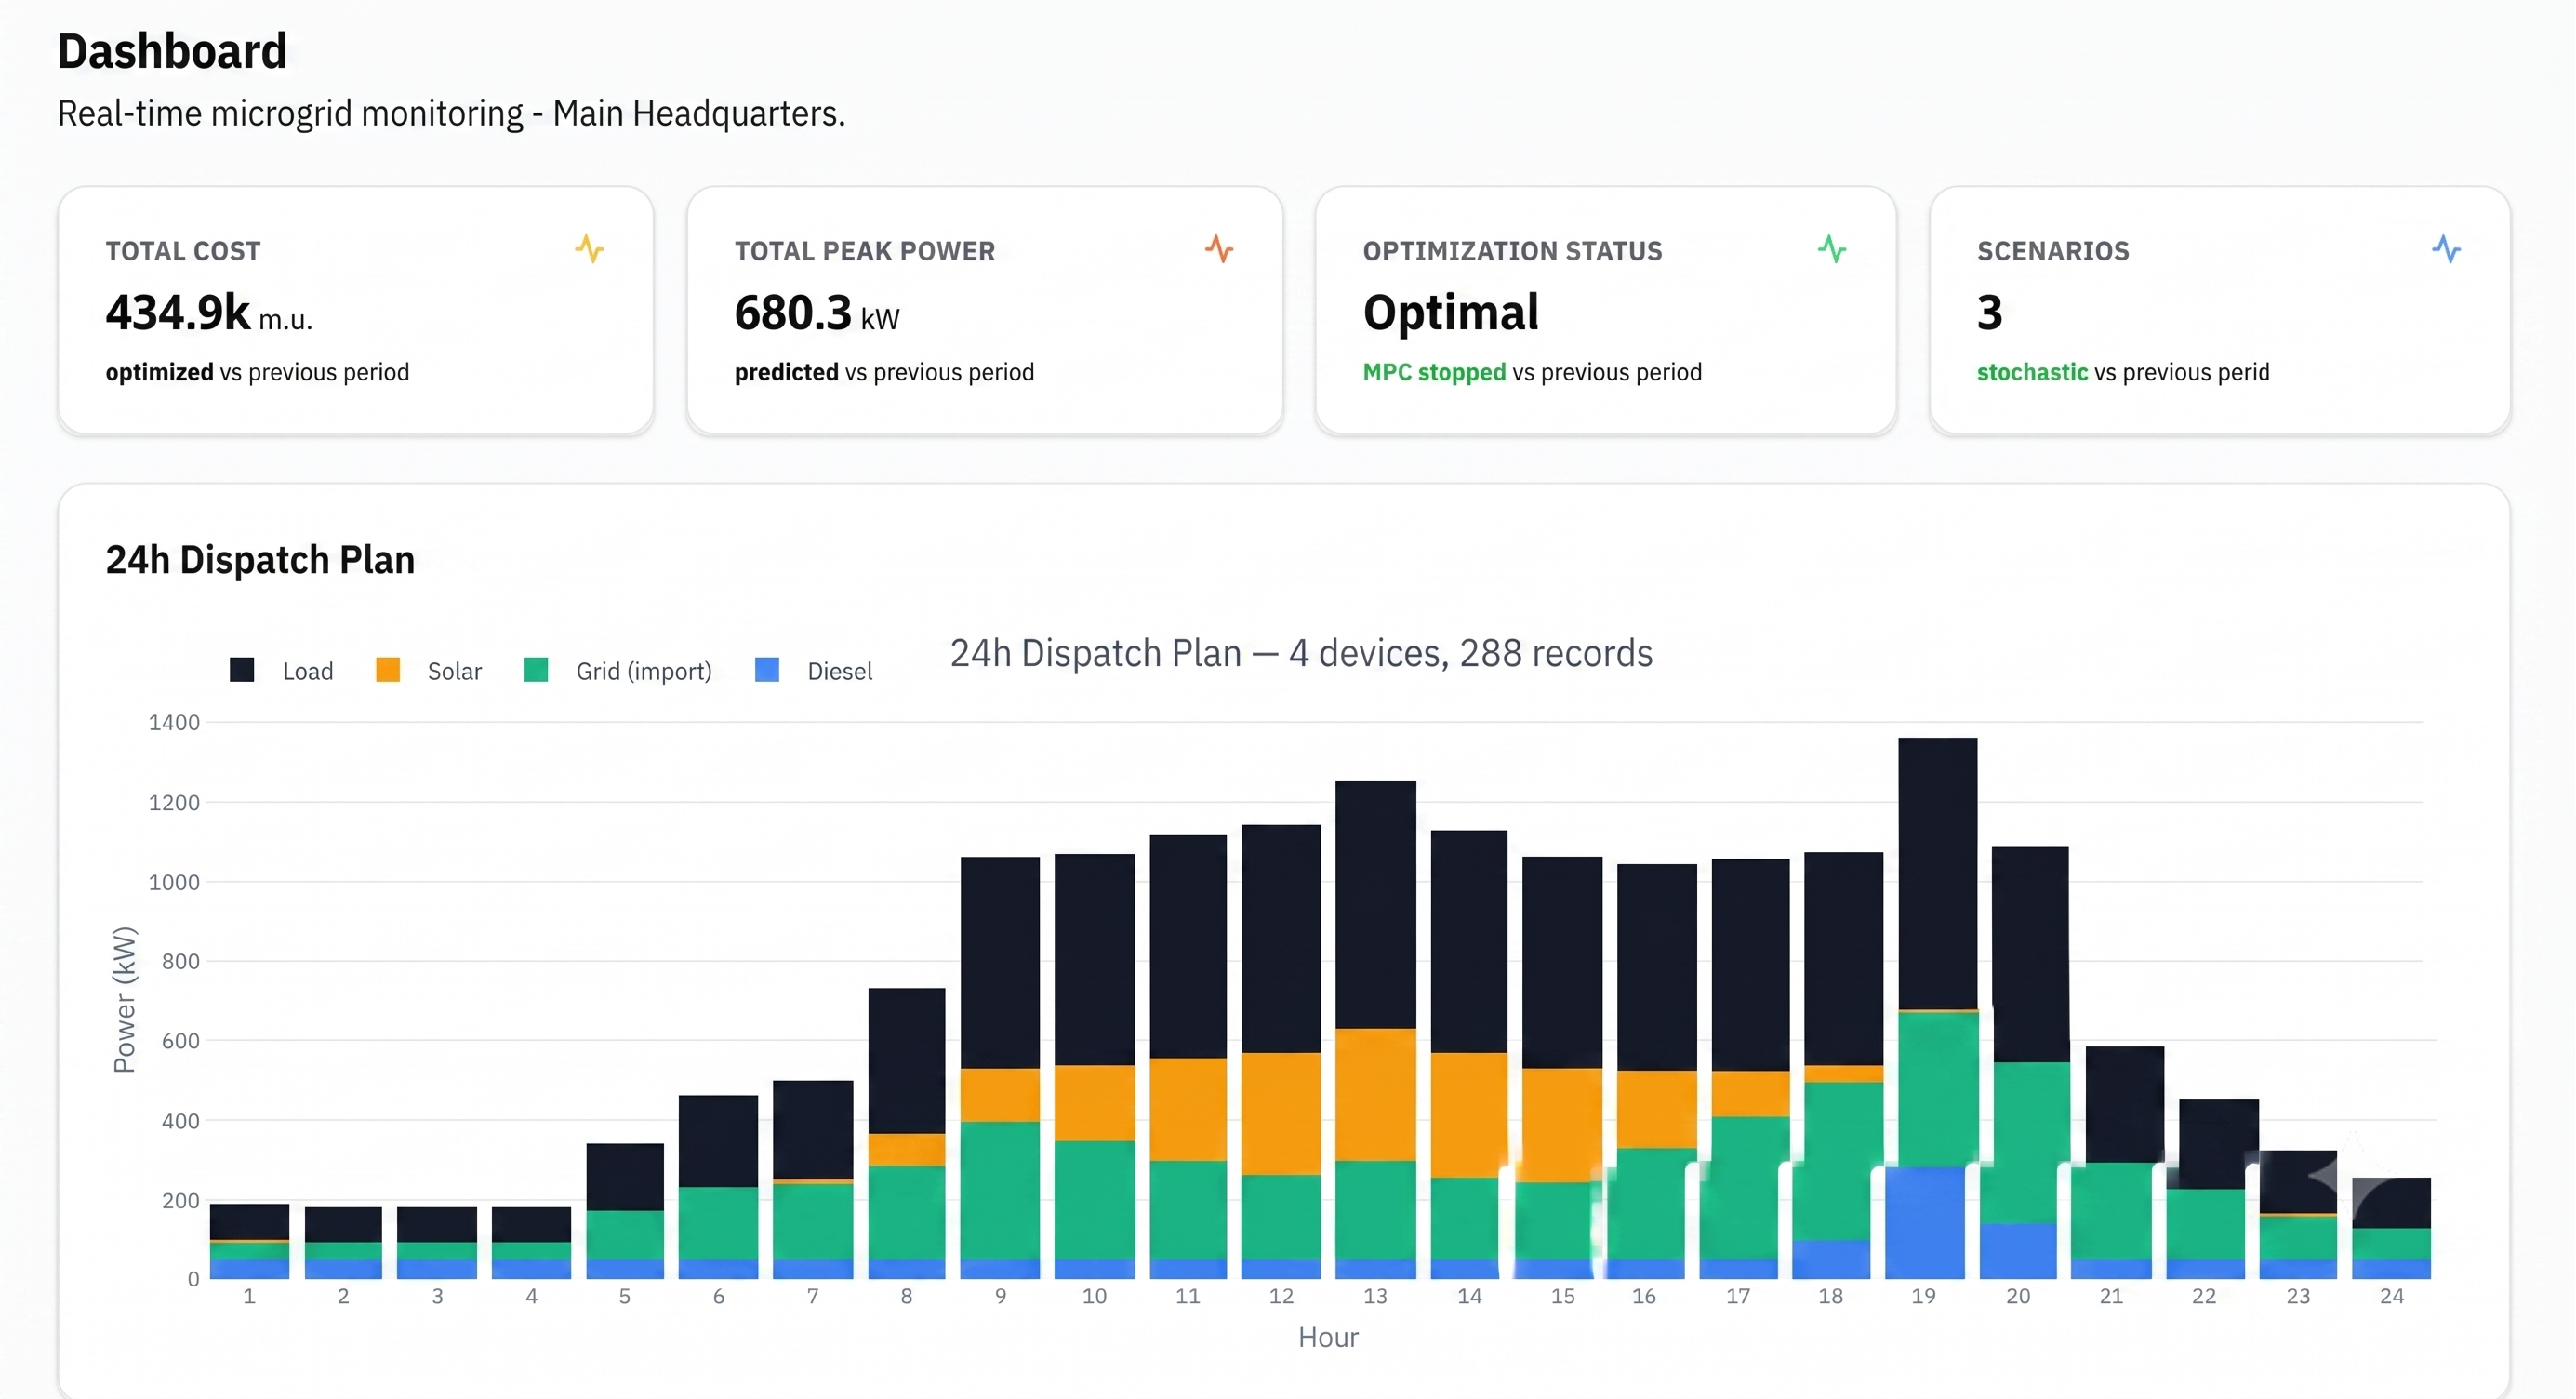
\includegraphics[width=\textwidth]{ENGimages/ui_dashboard_despacho.png}
    \caption{Optimization cycle result using MPC for a 24-hour horizon.}
    \label{fig:dashboard_opt}
\end{figure}

The obtained dispatch plan satisfies the projected demand by distributing the power among the available resources according to the model's operational constraints. Figure~\ref{fig:kpis} summarizes the main indicators generated after each execution of the MPC cycle.

\begin{figure}[H]
    \centering
    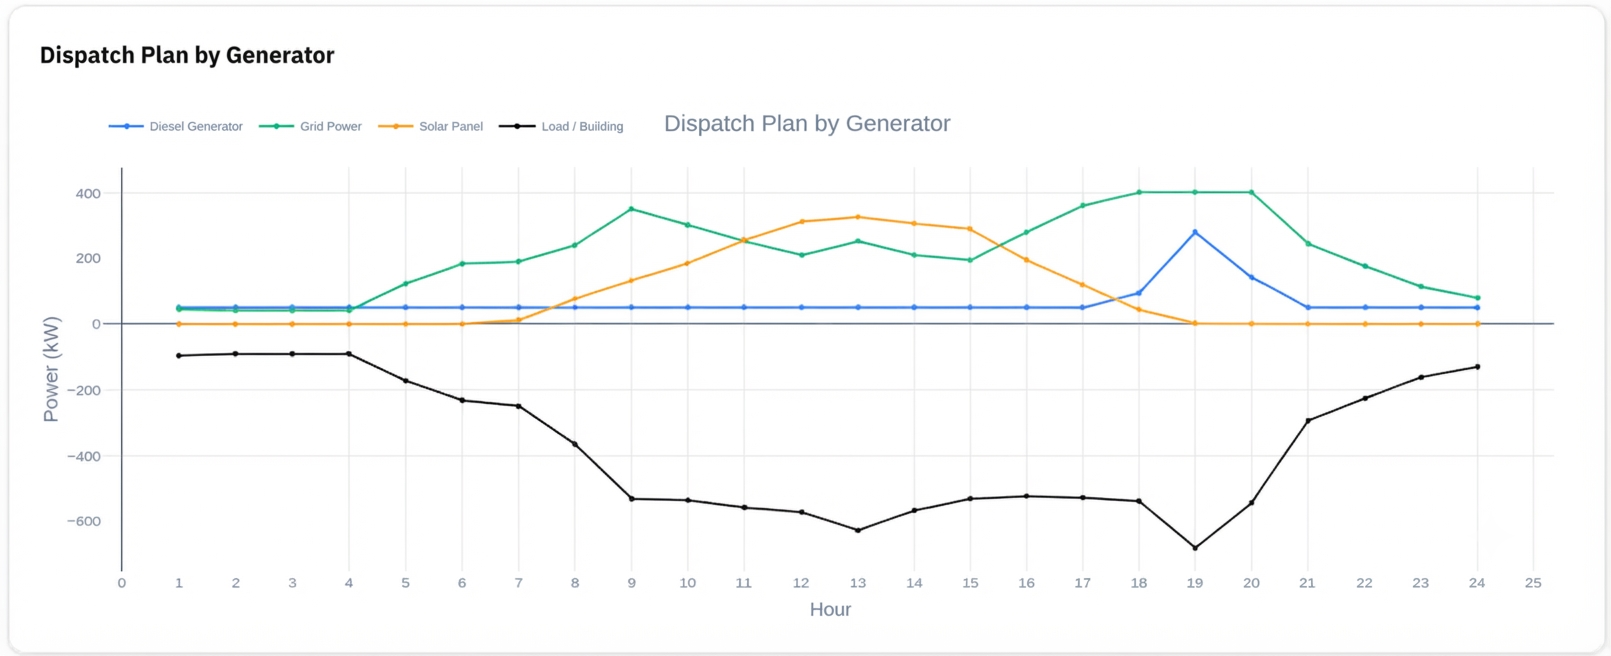
\includegraphics[width=0.85\textwidth]{ENGimages/resultados_despacho.png}
    \caption{Indicators obtained after the execution of the optimization cycle.}
    \label{fig:kpis}
\end{figure}

The calculated indicators include the total operation cost, the maximum power dispatched, and the optimization process status. These metrics allow monitoring the system's behavior during each iteration of the receding horizon implemented by the MPC. These results correspond to the optimization process; however, this process depends on the availability of forecasts for the energy variables considered by the model.

Figure~\ref{fig:tft} presents the behavior of the Temporal Fusion Transformer model during the offline training phase. Figure~\ref{fig:tft}(a) compares the real and predicted solar generation, while Figure~\ref{fig:tft}(b) presents the comparison between the real and estimated values for the voltage of phases A and B.

\begin{figure}[H]
    \centering
    % Subfigura (a) - Generación Solar (Arriba)
    \subfloat[Solar generation\label{fig:tft_solar}]{%
        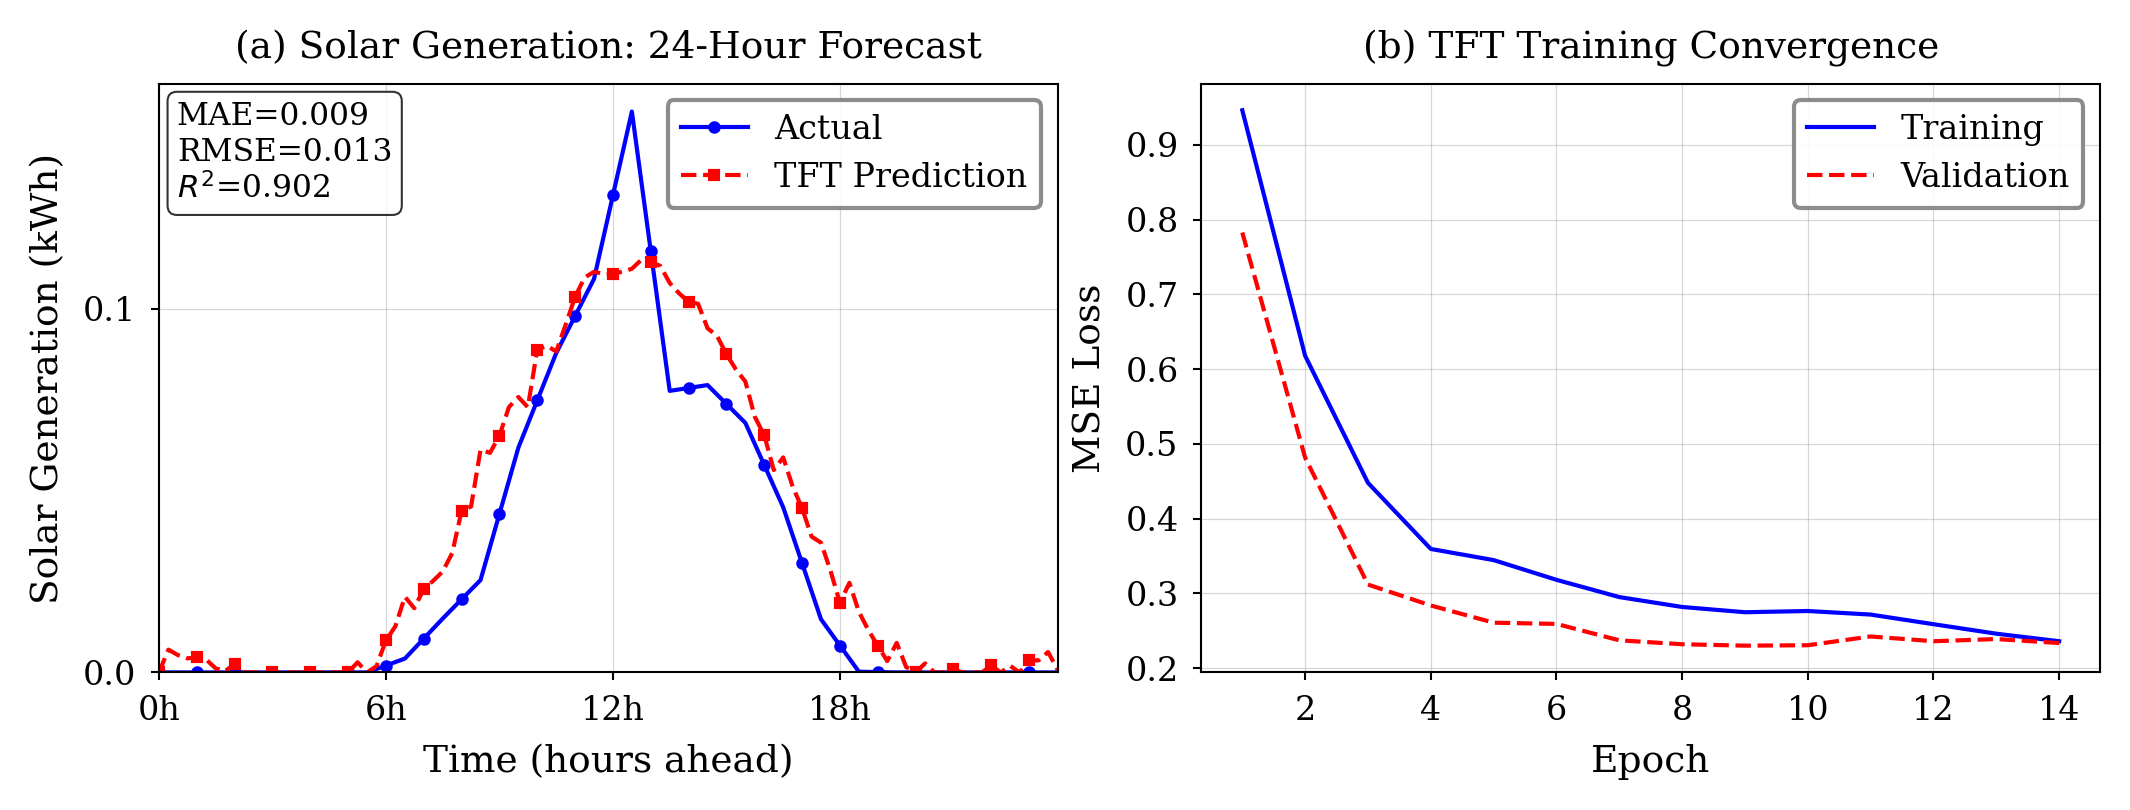
\includegraphics[width=0.75\textwidth]{images/tft_pred_solar.png}%
    }
    
    \vspace{0.5cm} % Añade un espacio vertical de separación entre las dos imágenes
    
    % Subfigura (b) - Voltaje (Abajo)
    \subfloat[Voltage\label{fig:tft_carga}]{%
        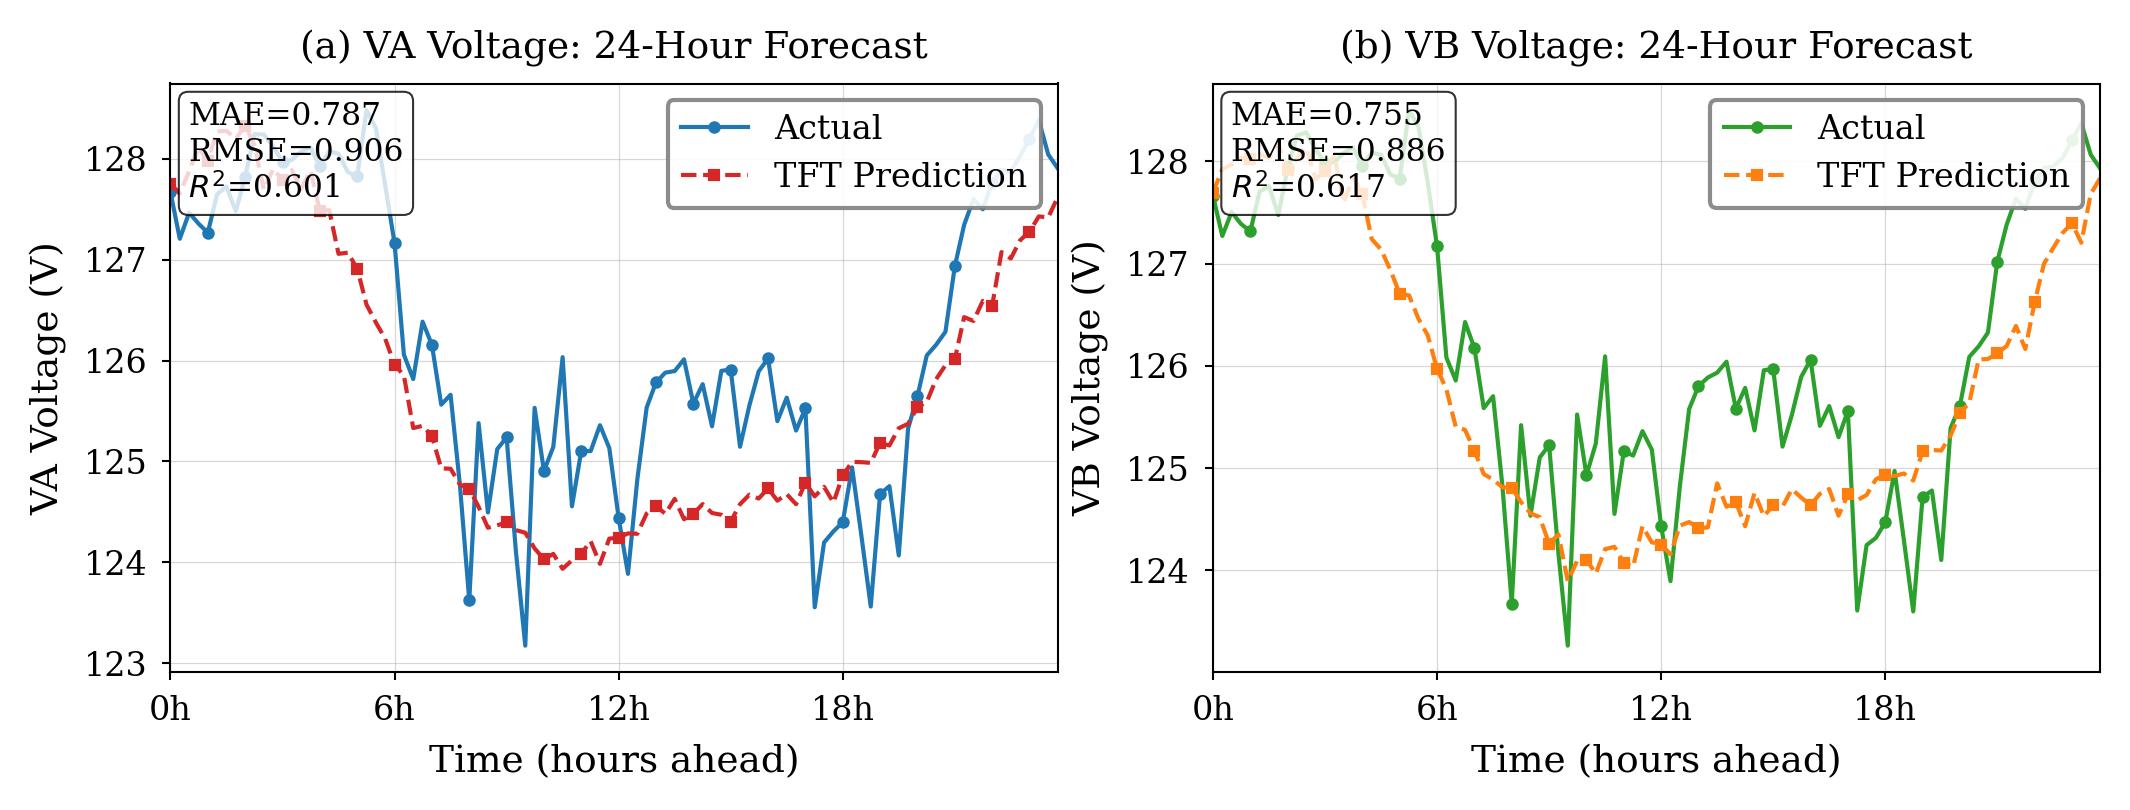
\includegraphics[width=0.75\textwidth]{images/tft_pred_carga.png}%
    }
    
    \caption{Comparison between measurements and predictions obtained using the TFT model.}
    \label{fig:tft}
\end{figure}

The predictions reproduce the general trend observed in the analyzed variables and keep most of the observations within the uncertainty intervals estimated by the model. In addition to the evaluation of the optimization model and the predictor, the functional integration of the different components that make up SIGE was verified.

The platform continuously receives information from IoT meters via MQTT, stores the measurements in MongoDB, executes the optimization processes, and updates the operator interface via WebSockets. Complementarily, the system incorporates modules for real-time monitoring, dynamic dashboard generation, and operator assistance through a multi-agent system based on language models.

To substantiate the real-time operation claims, this section reports the system performance metrics measured on the deployment environment. A reproducible benchmark suite measures the end-to-end latency and throughput of each communication and computation stage; the hardware and software stack used for the measurements are declared so that the results can be reproduced.

\begin{table}[H]
    \centering
    \caption{System performance metrics (measured on the deployment environment).}
    \label{tab:performance}
    \begin{tabular}{llccc}
        \toprule
        \textbf{Subsystem} & \textbf{Metric} & \textbf{p50} & \textbf{p95} & \textbf{p99} \\
        \midrule
        MQTT (end-to-end)   & publish $\rightarrow$ receive latency (ms) & 248.5 & 295.4 & 298.2 \\
        MQTT (throughput)   & sustained messages/s                     & \multicolumn{3}{c}{99.4} \\
        MongoDB (insert)    & write latency (ms)                       & 1001.1 & 2004.0 & 2004.0 \\
        MongoDB (throughput)& writes/s                                   & \multicolumn{3}{c}{380.1} \\
        MPC solver (LP relax) & solve time per 24 h cycle (ms)        & 24.8 & 101.8 & 101.8 \\
        MPC solver (Gurobi MIQP) & solve time per 24 h cycle (ms)    & -- & -- & -- \\
        WebSocket (push)    & backend $\rightarrow$ frontend latency (ms) & 1.2 & 1.4 & 5.6 \\
        REST API            & requests/s (50 connections)              & \multicolumn{3}{c}{10770} \\
        \bottomrule
    \end{tabular}
\end{table}

The model construction step (Pyomo model assembly for a 24-hour horizon with three weather scenarios and one battery) was measured at approximately 10 ms on the test machine, indicating that the formulation overhead is negligible compared to the solver time. With the free HiGHS solver, the continuous LP relaxation of the dispatch problem (binaries relaxed, quadratic cost linearized) solves in approximately 24.8 ms (p50), 101.8 ms (p95) and 101.8 ms (p99) for a 24-hour horizon, well within the 15-minute recalculation interval of the MPC. The exact MIQP solve time with a commercial Gurobi license is reported in Table~\ref{tab:performance}; the LP-relaxation figure provides a conservative lower bound that confirms the solver stage is not the bottleneck of the closed loop. The absolute values depend on the specific hardware and solver license. The remaining end-to-end metrics were populated by executing the provided benchmark scripts on the target deployment and are summarized in Table~\ref{tab:performance}: the MQTT broker (remote) exhibits an end-to-end publish-to-receive latency of 248.5 ms (p50), 295.4 ms (p95) and 298.2 ms (p99) at a sustained throughput of 99.4 messages/s; the MongoDB write path (remote cluster) shows an insert latency of 1001.1 ms (p50), 2004.0 ms (p95) and 2004.0 ms (p99) at a sustained throughput of 380.1 writes/s for the measured batch size; the REST API sustains about 10,770 requests/s under 50 concurrent connections, with a latency of 4 ms (p50), 4 ms (p95) and 10 ms (p99), limited by the JWT validation round-trip; and the Socket.IO push channel (backend to frontend) exhibits a latency of 1.2 ms (p50), 1.4 ms (p95) and 5.6 ms (p99) measured over 20 optimization-start events. The exact MIQP solve time under a commercial Gurobi license remains the only unmeasured cell and is left as future work.

The integrated operation of these components allowed the complete cycle of data acquisition, processing, optimization, and visualization to be executed within the proposed architecture, verifying the communication among the different implemented services.
%%%%%%%%%%%%%%%%%%%%%%%%%%%%%%%%%%%%%%%%%%

\section{Discussion}
The results obtained show the viability of the proposed architecture to integrate data acquisition, prediction, optimization, and operator assistance processes into a single platform. Rather than independently evaluating each of these components, the validation performed demonstrates the system's ability to coordinate their operation through a decoupled architecture based on specialized services.
\\
\\
One of the platform's main contributions corresponds to the modular design of the prediction system. The implementation of an abstract interface alongside a FastAPI-developed API decouples the forecasting engine from the rest of the architecture, allowing the incorporation or substitution of different models without modifying the backend orchestration flow. This decision facilitates the platform's evolution as new algorithms or more representative datasets become available.
\\
\\
In this architecture, the Temporal Fusion Transformer model constitutes an implementation developed to validate the incorporation of advanced prediction models within the platform. Because the training was conducted using an independent pipeline and utilizing a dataset corresponding to an initial microgrid operation stage, the current validation is oriented toward demonstrating the architecture's readiness for integration rather than performing an exhaustive evaluation of predictive performance.
\\
\\
Currently, the MPC cycle operates using the historical series-based predictor implemented in Matlab, while the TFT model remains decoupled from the production environment until its validation process is completed. Thanks to the modular design implemented via the prediction API, the incorporation of the new model can be carried out without modifying the rest of the system's architecture.
\\
\\
Finally, the multi-agent system based on LLMs processed the outputs of the statistical anomaly detector and generated structured responses in natural language. However, the verification of these diagnostics was restricted to structural compliance with Zod schemas, without including a quantitative evaluation of the technical accuracy of the recommendations, such as the false-positive rate, real fault coverage, or response latency, nor a measurement of the perceived utility by human operators. Validating the system's effectiveness as an assistance tool requires a controlled study with operators contrasting actions taken with and without the AI agent's support.  
\\

%%%%%%%%%%%%%%%%%%%%%%%%%%%%%%%%%%%%%%%%%%
\section{Conclusions}
In this work, SIGE was developed and validated, a modular platform for the intelligent management of microgrids that integrates IoT monitoring, optimization via MPC, and operator assistance tools within a decoupled and extensible architecture. The platform demonstrates that it is feasible to operate a hybrid microgrid autonomously through MPC cycles, combining mathematical optimization with intelligent real-time analysis.

From a functional point of view, the platform proved capable of processing data flows from IoT sensors in real-time, updating operator visualizations with reduced latencies and automatically generating optimization model constraints from the topology defined in the single-line diagram editor. The communication architecture between the service orchestrator and the optimization engine, based on job queues with periodic polling, completed prediction and dispatch cycles at 15-minute intervals, suggesting that the platform is applicable to operational environments with intra-hour response times.
\\

Future work proposes completing the integration of the Temporal Fusion Transformer model into the operational cycle of SIGE, allowing the forecasts generated by the prediction engine to automatically feed the predictive control scheme. Similarly, it is planned to evaluate the platform using larger datasets and different microgrid configurations, as well as to incorporate new prediction models taking advantage of the implemented modular design.


\vspace{6pt}
%%%%%%%%%%%%%%%%%%%%%%%%%%%%%%%%%%%%%%%%%%
\acknowledgments{
The authors acknowledge the support of the research project "Desarrollo de una solución tecnológica para el análisis de flujos de potencia en redes eléctricas de distribución desbalanceadas con generación distribuida" ID-3214, supported by Agreement No. 29, dated January 17, 2025, by VIIS of the Universidad de Nariño. We also thank the Department of Electronic Engineering and the Electrical and Electronic Engineering Research Group (GIIEE) at the Universidad de Nariño for their support of the academic and administrative processes necessary to carry out this project.
}

\conflictsofinterest{The authors declare no conflicts of interest related to this scientific development.}
\dataavailability{The source codes and data of the TFT model will be structured as closed institutional repositories pending formal scientific licensing guidelines.}
%%%%%%%%%%%%%%%%%%%%%%%%%%%%%%%%%%%%%%%%%%
\begin{adjustwidth}{-\extralength}{0cm}
\reftitle{References}
\begin{thebibliography}{999}
\bibitem{ref-lim}
Lim, B., Arik, S. O., Loeff, N., \& Pfister, T. Temporal Fusion Transformers for interpretable multi-horizon time series forecasting. \textit{International Journal of Forecasting}, \textbf{2021}, \textit{37}(4), 1748-1764.

\bibitem{ref-bynum}
Bynum, M. L., Hackebeil, G. A., Hart, W. E., Laird, C. D., Nicholson, B. L., Siirola, J. D., Watson, J. P., \& Woodruff, D. L. \textit{Pyomo --- Optimization Modeling in Python}, 3rd ed.; Springer, 2021.

\bibitem{ref-gurobi}
Gurobi Optimization, LLC. Gurobi Optimizer Reference Manual. \textbf{2024}.

\bibitem{ref-rawlings}
Rawlings, J. B., Mayne, D. Q., \& Diehl, M. M. \textit{Model Predictive Control: Theory, Computation, and Design}, 2nd ed.; Nob Hill Publishing, 2017.

\bibitem{ref-birge}
Birge, J. R., \& Louveaux, F. \textit{Introduction to Stochastic Programming}, 2nd ed.; Springer, 2011.

\bibitem{ref-huangfu}
Huangfu, Q. \& Hall, J. A. J. Parallelizing the dual revised simplex method. \textit{Mathematical Programming Computation}, \textbf{2018}, \textit{10}(1), 119-142.

\bibitem{ref-chase}
Chase, H. \textit{LangChain: Building applications with LLMs through composability}. \textbf{2022}.

\bibitem{ref-alternar}
Pantoja, A., Fajardo, D., \& Revelo, J. ALTERNAR: An\'alisis de Oportunidades Energ\'eticas con Fuentes Alternativas en el Departamento de Nari\~no. \textit{Premio AMBAR 2016}, \textbf{2016}.

\bibitem{ref-rao}
Rao, C. K., Sahoo, S. K., \& Yanine, F. F. A literature review on an IoT-based intelligent smart energy management systems for PV power generation. \textit{Hybrid Advances}, \textbf{2024}, \textit{5}, 100136.

\bibitem{ref-tasmant}
Tasmant, H., Bossoufi, B., Alaoui, C., \& Siano, P. A review of machine learning and IoT-based energy management systems for AC microgrids. \textit{Computers and Electrical Engineering}, \textbf{2025}, \textit{127}, 110563.

\bibitem{ref-lami}
Lami, B., Alsolami, M., Alferidi, A., \& Slama, S. B. A Smart Microgrid Platform Integrating AI and Deep Reinforcement Learning for Sustainable Energy Management. \textit{Energies}, \textbf{2025}, \textit{18}(5), 1157.

\bibitem{ref-medicion}
Arciniegas M., A. F., Imbajoa R., D. E., \& Revelo F., J. Dise\~no e implementaci\'on de un Sistema de Medici\'on Inteligente para AMI de la microrred de la Universidad de Nari\~no. \textit{Enfoque UTE}, \textbf{2017}, \textit{V.7-Sup.1}, 300--314.

\bibitem{ref-carrasco}
Carrasco, F., Kristjanpoller, F., Verdugo, I., Viveros, P., \& Pascual, R. Forecast-informed daily energy dispatch for cost and emission reduction: Evidence from an emerging economy power system. \textit{Energy Convers. Manag.}, \textbf{2026}, \textit{364}, 121611.

\bibitem{Parisio2014}
A.~Parisio, E.~Rinaldi, y L.~Glielmo, ``Model predictive control of microgrids'', \emph{IEEE Transactions on Control Systems Technology}, vol. 22, no. 5, pp. 1622--1628, 2014.

\bibitem{Su2014}
W.~Su, J.~Wang, y J.~Roh, ``Stochastic energy management for a microgrid with renewable energy resources and energy storage systems'', \emph{IEEE Transactions on Smart Grid}, vol. 5, no. 4, pp. 1747--1755, 2014.

\bibitem{Zia2018}
M.~F.~Zia, E.~Elbouchikhi, y M.~Benbouzid, ``Microgrids energy management systems: A critical review on methods, solutions, and prospects'', \emph{Applied Energy}, vol. 222, pp. 1033--1055, 2018.

\bibitem{Hua2019}
H.~Hua, Y.~Qin, C.~Hao, y J.~Cao, ``Optimal energy management strategies for energy Internet via deep reinforcement learning approach'', \emph{Applied Energy}, vol. 239, pp. 598--609, 2019.

\bibitem{Han2026}
W.~Han, J.~Cui, X.~Wang, y X.~Chen, ``Resilient Optimal Dispatch of Ship-Integrated Energy System and Air Lubrication Using an Enhanced Traffic Jam Optimizer'', \emph{Journal of Marine Science and Engineering}, vol.~14, no.~9, p.~779, 2026.

\end{thebibliography}
\PublishersNote{}
\end{adjustwidth}
\end{document}